\input{../Test/top-apj}



% Headers for odd and even pages, respectively:
\shorttitle{Homework 1: Variable Stars}
% If more than two authors, use {\em et al.}
\shortauthors{Francisco F. Carrasco Varela}


\begin{document}

\title{Homework 1: Variable Stars}

\author{Francisco Carrasco Varela\altaffilmark{1}
}

\affil{\sp{1} Astronomy Student. Pontificia Universidad Catolica de Chile, Instituto de Astrofisica.  Av. Vicuna Mackenna 4860,
782-0436 Macul, Santiago, Chile.\\}

\email{ffcarrasco@uc.cl}

\begin{abstract}
  This homework is based on 
  \href{https://uploadfiles.io/g9bzu}
  {Marcio Catelan's first homework.} First, I show a little approximation about General Catalog of Variable Stars (GCVS) and its content. Second, a little overview about a computer program for binary stars: \texttt{Phoebe}; how it works and what can we do with it. Third, given magnitudes for two variables stars in function of time (which are ground-based data) I compute their period using \texttt{Period04} program; giving $P_1 = 0.866062 d$ for first star (classified by me as an eclipsing variable) and $P_2 = 0.486062 d$ for the second (classified by me as an eruptive variable). Fourth and last, I compute the period for variable stars as mentioned in the third item; but now the difference is this variable stars are spaced-based observed; also finding one of them is a multiperiodic variable. 

\end{abstract}

% http://journals.aas.org/authors/keywords2013.html
\keywords{catalog: GCVS -- program: Phoebe --- program: Period04 ---
          variable stars}


\section{First Problem: General Catalog of Variable Stars (GCVS)}
\label{p1}

Here I'm going to work with the GCVS. This is a catalog which is a compilation of variability data that has appeared in the literature. I'm going to work with the \emph{updated} one version, i.e., version 5.1 (updated version when this homework was done); which have been updated in March, 2017. 

\begin{enumerate} [a)]
\item As we have seen in class, variable stars (and objects) may be classified according to their astrophysical reason for variability. In GCVS variable objects have been classified in: \texttt{i)} Eruptive, \texttt{ii)} Pulsating, \texttt{iii)} Rotating, \texttt{iv)}Cataclysmic (novalike \& explosive), \texttt{v)} Eclipsing binary systems, \texttt{vi)} Intense variable X-ray sources, \texttt{vii)} Other symbols and, finally, \texttt{viii)} New variability types.

For purpouses of this homework, I will work with the first five types of variability named above (i.e., from \texttt{i)} to \texttt{v)}).

Based on \href{http://adsabs.harvard.edu/abs/2017ARep...61...80S}
  {Samus et al. 2017.} (hereafter, S17) paper, who used GCVS 5.1 version (so it's updated), gave an estimated number of each variability stars-objects. This can be easily found too in \href{http://www.sai.msu.su/gcvs/gcvs/gcvs5/vartype.htm}{GCVS official website}, which is based in the same paper cited previously. A \href{http://www.sai.msu.su/gcvs/gcvs/gcvs5/gcvs5.txt}{GCVS file} can be downloaded, read and make a summary; comparable with the results given by S17. Before continue, \href{http://www.sai.msu.su/gcvs/gcvs/gcvs5/}{some usual files can be found in GCVS webpage}. Being consistent with the roman enumeration above, I have chosen the next type of variabilities (e.g. \texttt{i)} means this is an Eruptive type variability): \texttt{i)} UV (Eruptive variable of the UV Ceti type) , \texttt{ii)} RR (variable RR Lyrae type), \texttt{iii)} SXARI (SX Arietis-type variables), \texttt{iv)} N (Novae) and, last, \texttt{v)} E (Eclipsing binary systems).
  
My results and results shown by S17 are given in Table 1 and also in Fig. 1. The difference between my results and results given by S17 may settle in how we read \href{http://www.sai.msu.su/gcvs/gcvs/gcvs5/gcvs5.txt}{the data}. Personally, the \texttt{.txt} file given by GCVS staff is in a terrible structure and it's not ``trivial'' to read (comparing it with others data-tabled that I have read, like APOGEE).

\begin{table}[ht]
\centering
\caption{\label{table:parameters} Counts for variability subclasses objects; comparing results found by me with results found by S17. As said, all the counts are, approximately, in the same order of magnitude.}
\begin{tabular}{lcr}
\hline
\hline
Variable subclass                          & My counts & S17 counts     \\
\hline
 UV        &       996 & 997\\
 RR & 1357 & 1440 \\
 SXARI & 26 & 25 \\
 N & 64 & 61 \\
 E & 478 & 479 \\
\hline
% SOURCE: /home/patricio/ast/esp01/analyses/ligtcurve/attempt_547/results.txt
\end{tabular}
\end{table}

\begin{figure}[tb]
\centering
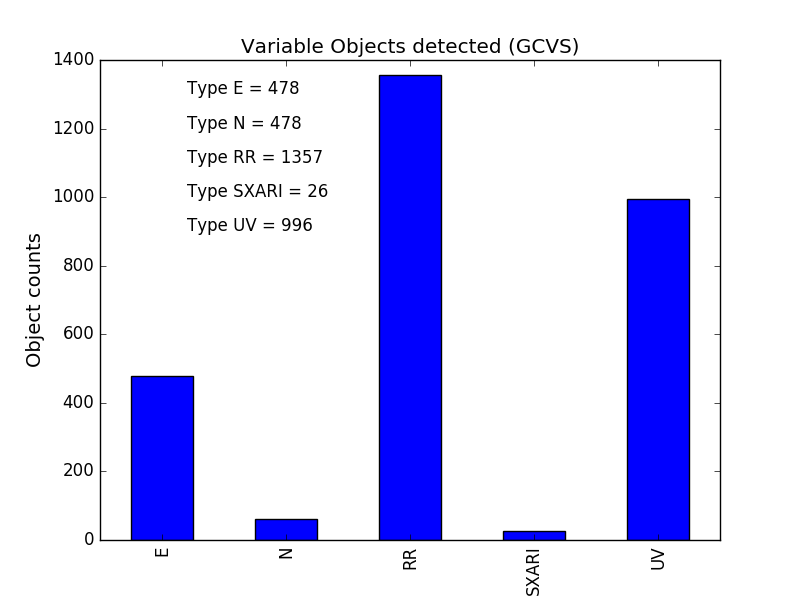
\includegraphics[width=\linewidth, clip]{Histograma_subclass.png}
\caption{Histogram of variability subclasses. This histograms shows counts for UV, RR, SXARI, N \&  E subclasses. Even when I chose subclasses randomly, RR subclass has, by far, the larger number of counts; followed by UV subclass.}
\label{fig:F1}
% SOURCE: /home/patricio/ast/esp01/code/lib/python/xkcd/paperwritting.py
\end{figure}
  
\item A \href{http://www.sai.msu.su/gcvs/gcvs/constel.txt}{Constellation numeric code} can be also found in GCVS webpage. Host constellations can be obtained from \href{http://www.sai.msu.su/gcvs/gcvs/gcvs5/gcvs5.txt}{\texttt{gcvsr.txt}}. Python code for this (and for all this homework) can be found in \href{https://github.com/Panchitoz1/Estrellas_Variables}{Github}. The result is shown in Fig. 3 as a histogram and in Table 2.

\begin{figure}[tb]
\centering
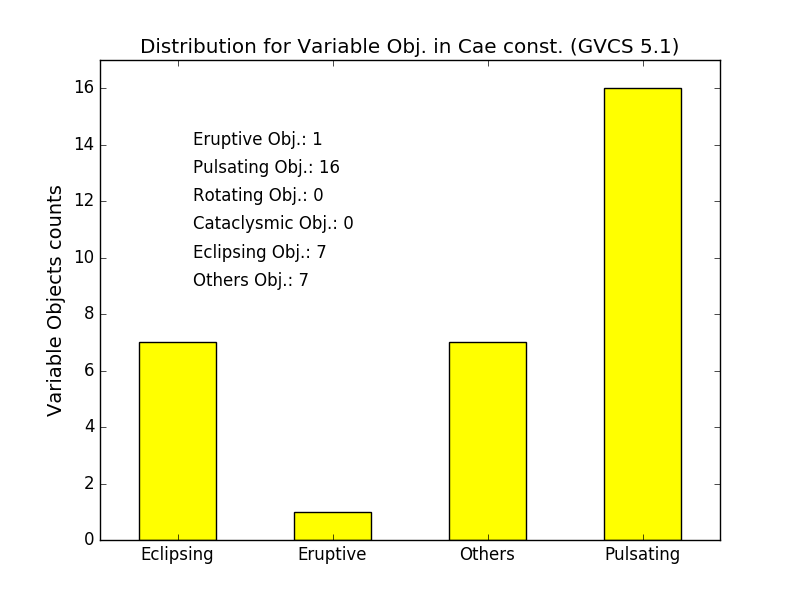
\includegraphics[width=\linewidth, clip]{Cae_variable_dist.png}
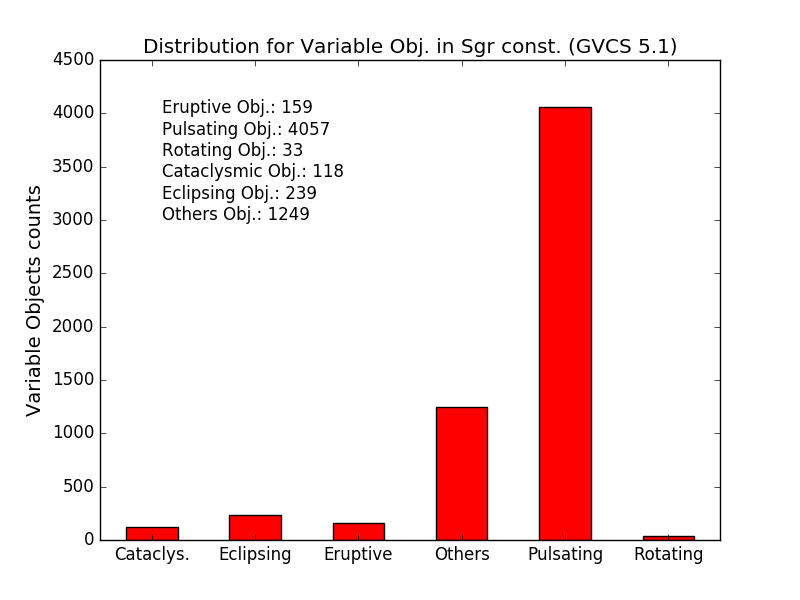
\includegraphics[width=\linewidth, clip]{Sgr_variable_dist.png}
\caption{\textit{Top}: Distribution for Variable Objects in Cae constellation.
\textit{Bottom}: Distribution for Variable Objects in Sgr constellation.
Even when the sample of both constellations is very unequal they have similarities: they both contain, in a high percentage, pulsating objects; and in a low percentage cataclysmic and rotating objects.}
\label{fig:F1}
% SOURCE: /home/patricio/ast/esp01/code/lib/python/xkcd/paperwritting.py
\end{figure}

\begin{figure*}
\centering
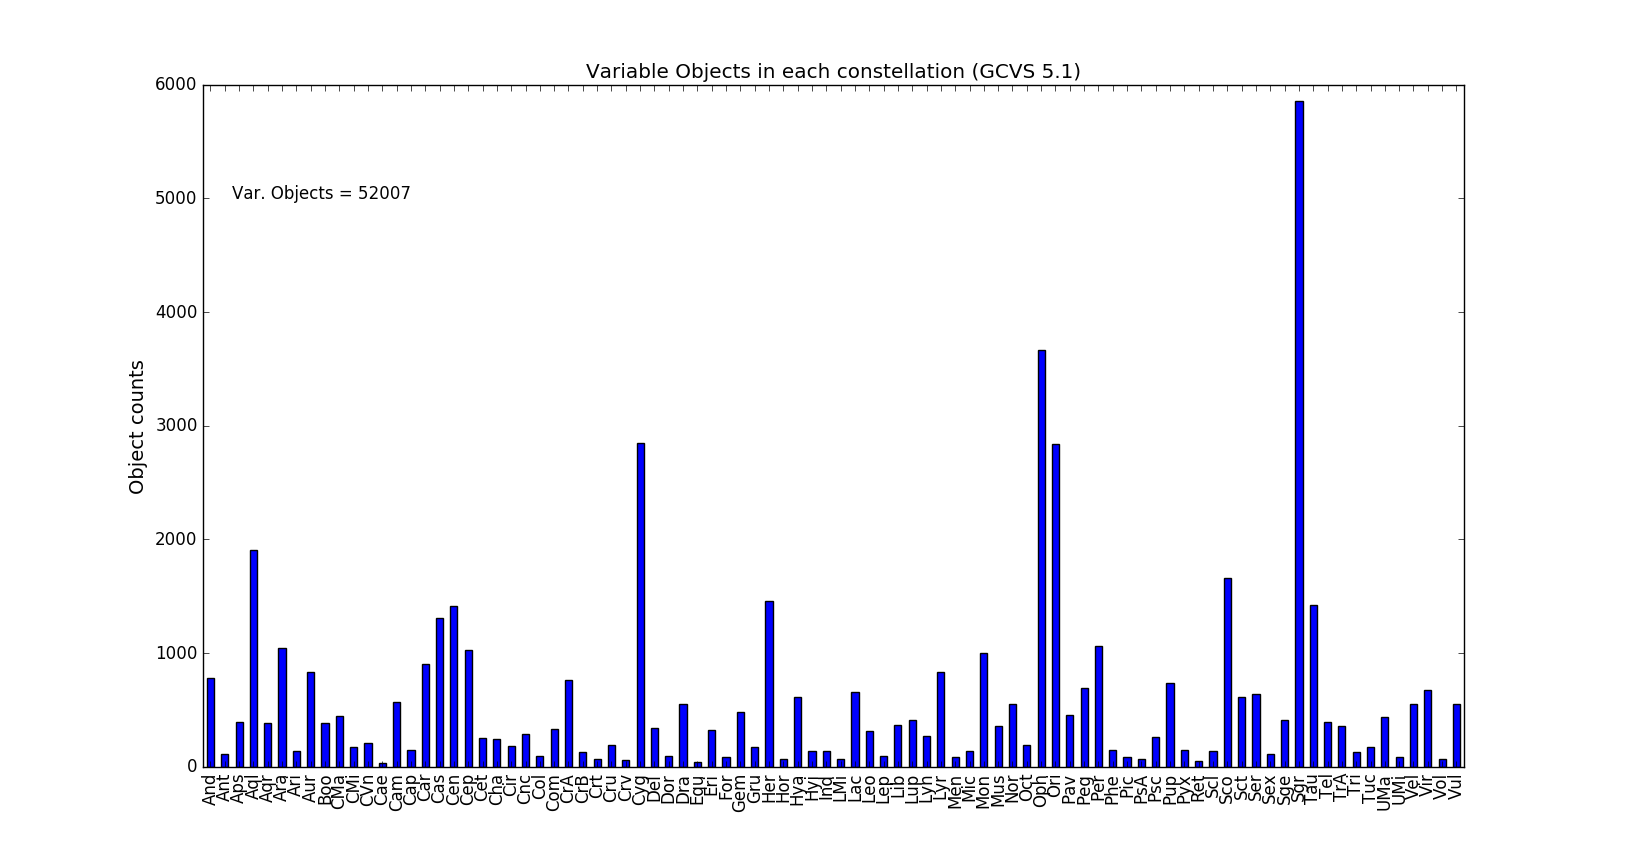
\includegraphics[width=\linewidth, clip]{Histograma_constelaciones.png}
\caption{Histogram for variability objects in constellations. This histogram shows variable objects detected for the 88 constellations present in GCVS 5.1.}
\label{fig:F1}
% SOURCE: /home/patricio/ast/esp01/code/lib/python/xkcd/paperwritting.py
\end{figure*}

\begin{table}[ht]
\centering
\caption{\label{table:parameters} Some constellations with their numbers of variable objects. This table shows, specifically, those constellations with a larger and a smaller numbers of variable objects found. Numbers in parenthesis are their order in GCVS, which is ordered alphabetically (i.e., (1) is Andromeda and (88) is Vulpecula).}
\begin{tabular}{lc}
\hline
\hline
Constellation                          & Variable Objects Number        \\
\hline
(72)Sgr              &       5855 \\
(59)Oph           & 3665          \\
(31)Cyg           & 2848          \\
(60)Ori & 2839 \\
(28)Crv & 55 \\
(70)Ret & 53 \\
(35)Equ & 44 \\
(10)Cae & 31 \\
\hline
% SOURCE: /home/patricio/ast/esp01/analyses/ligtcurve/attempt_547/results.txt
\end{tabular}
\end{table}



\item As shown in Table 2, Sgr constellation has the largest number of Variable Objects in GCVS 5.1; while Cae has the smallest. Here I'm going to show, approximately, how 	do the stars distribute in this constellations considering their class of variability as the selection criteria. With ``class of variability'' I mean those explained with roman numbers in subitem \texttt{a)} of the first problem of this homework, focusing on the first five; for those variable stars/objects that are not considered (simply because my software doesn't get them) I decided to classify them as ``Others''. But, caution; for example, subclass for eclipsing binary systems called in GCVS as ``E/WD'' is not considered as an eclipsing variable in my program; instead, it is considered in ``Others''. Sadly, I had to do this because there are a lot of combinations of subclasses. Also, sometimes GCVS has some special symbols for their stars such like $+$ or $*$ (if the reader doesn't know what I'm talking about, it is highly recommendable to visit \href{http://www.sai.msu.su/gcvs/gcvs/gcvs5/vartype.htm}{GCVS Variables homepage}. For example, $+$ symbol means a variable star belongs to a several type of light variability simultaneously; e.g., E+RR is an eclipsing/RR type variable star). That's why ``Other type'' stars in Tables 3 contain (and I'm sure about that) eclipsing, rotating, pulsating, cataclysmic and eruptive variables; and they show, actually, a larger number than they should be. This distribution can also be appreciated in Figure 2 as a histogram for both constellations.

\begin{table}[ht]
\centering
\caption{\label{table:parameters} Counts for variability classes objects. The reader can check that the number of total stars is the same in this Table and in Table 2.}
\begin{tabular}{lcr}
\hline
\hline
Variable class                          & Sgr counts & Cae counts     \\
\hline
 Eruptive  &  159   &  1 \\
 Pulsating & 4057 & 16 \\
 Rotating & 33 & 0 \\
 Cataclysmic & 118 & 0 \\
 Eclipsing & 239 & 7 \\
 Others & 1249 & 7 \\
\hline
 Total & 5855 & 31 \\
\hline
% SOURCE: /home/patricio/ast/esp01/analyses/ligtcurve/attempt_547/results.txt
\end{tabular}
\end{table}



  
\end{enumerate} 

\section{Second Problem: PHOEBE}
\label{p2}

In this problem I'm going to use \texttt{PHOEBE} (PHysics Of Eclipsing BinariEs) software. It is quite popular among eclipsing binary community. Instead of use the old version suggested for this homework (2004 version), I'm using a newer one, \texttt{PHOEBE 2.0} through \texttt{Anaconda} (Python). Here, I'm going to mention what \texttt{PHOEBE} can do with a little description about it.

Everything explained here can be found in \href{http://phoebe-project.org/}{Phoebe Project Webpage}. Fortunately, it can be easily installed with \texttt{Anaconda}, as mentioned before (it is just a \texttt{sudo pip} command). 

What can compute \texttt{PHOEBE} with binary system? The following ones:

\begin{itemize}
\item detached and semi-detached roche binaries
\item keplerian orbits (including eccentric orbits with volume conservation)
\item passbands/atmospheres
\item limb darkening
\item gravity darkening
\item reflection (heating without redistribution)
\item finite integration time via oversampling
\item circular spots
\item contact systems (to mimic White Dwarfs)
\end{itemize}

Nevertheless, \texttt{PHOEBE 2.0} is a little bit ``new'' and has some disadvantages over \texttt{PHOEBE 1.0} (Physics unsupported at the moment) like:

\begin{itemize}
\item full support contact systems
\item semi-detached/single contact systems (planned future development)
\item  X-ray binaries
\end{itemize}

But, at the same time, it has advantages over \texttt{PHOEBE 1.0}:
\begin{itemize}
\item Doppler boosting
\item Single rotating stars
\item Lambert scattering


\end{itemize}

The next results have been obtained following the \href{phoebe-project.org/docs/2.0/#Tutorials}{\texttt{PHOEBE} tutorial} from its official webpage. I tried to make some plots using \texttt{UVLeo.phoebe} file, but for reasons that I still don't know \texttt{PHOEBE 2.0} shows an error when I try to load it.

So, here, I'm going to use the \texttt{phoebe. default\_binary()} configuration; loading ``dummy'' dataset based in \href{https://raw.githubusercontent.com/phoebe-project/phoebe2-docs/master/tutorials/test.lc.in}{\texttt{test.lc.in}} file that gives some properties to our binary systems (which consist, basically, in a binary system of 2 stars with 0.998 $M_{\odot}$ each one with an eccentricity of 0.1 and other parameters/dataset given in \texttt{PHOEBE 2.0} tutorial).  

For example, playing with our binary system I have simulated, with the binary system described above, binary system different trajectory axes. Also, \texttt{test.lc.in}, as mentioned, had some presetted dataset such like time, fluxes and their sigmas. With this we can play and make some plots. Some of this plots are presented in Fig 4. The rest of them are in \href{https://github.com/Panchitoz1/Estrellas_Variables}{my Github} with the codes used in this homework (check for PHOEBE\_notebook code if you want to see some more). I've played with \texttt{PHOEBE} changing axis units, axis limits, 3D plots, orbit axis plots, flux vs. time plots and others.

Here I only provide a little approximation to  \texttt{PHOEBE}. It is very useful to know, speciallly for the future, what can I do with it.

\begin{figure}[tb]
\centering
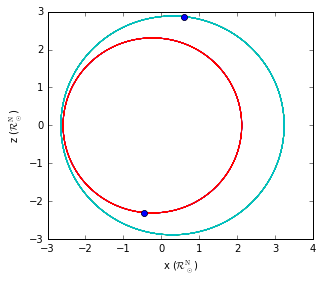
\includegraphics[scale=0.5]{Phoebe1.png}
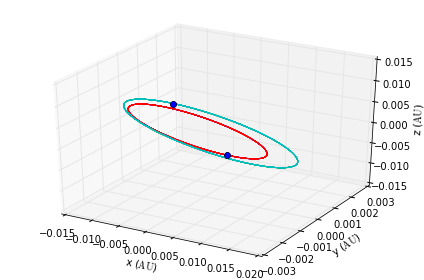
\includegraphics[scale=0.5]{Phoebe2.png}
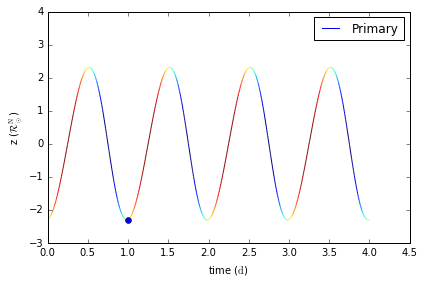
\includegraphics[scale=0.5]{Phoebe3.png}
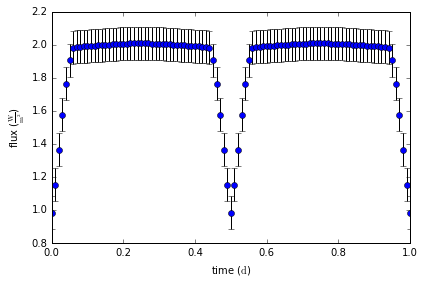
\includegraphics[scale=0.5]{Phoebe4.png}
\caption{Simulations obtained through \texttt{PHOEBE} with binary default system and defaults found in \href{https://raw.githubusercontent.com/phoebe-project/phoebe2-docs/master/tutorials/test.lc.in}{\texttt{test.lc.in}}. \textit{Top}: $z (R_{\odot}^N)$ vs. $x (R_{\odot}^N)$ orbits for a binary system. \textit{Middle-top}: 3D plot orbits for a binary system (with its units in $AU$). \textit{Middle-bottom}: $z(R_{\odot}^N)$ vs. time $(d)$. \textit{Bottom}: flux ($W \cdot m^{-2}$) vs. time $(d)$, with errorbars given in \href{https://raw.githubusercontent.com/phoebe-project/phoebe2-docs/master/tutorials/test.lc.in}{\texttt{test.lc.in}} file.} 
\label{fig:F1}
% SOURCE: /home/patricio/ast/esp01/code/lib/python/xkcd/paperwritting.py
\end{figure}

\begin{table}[ht]
\centering
\caption{\label{table:period04calc} Period and amplitudes calculated by \texttt{Period04} for \texttt{star1.txt} and \texttt{star2.txt}. Aparent magnitudes to compute this periods were in V band. (check Problem \ref{sec:p3}). Here I only show the first 6 decimals for reasons explained in Problem \ref{sec:p3}.}
\begin{tabular}{lcr}
\hline
\hline
File                          & Period ($d$) & Amplitude ($mag$)     \\
\hline
 \texttt{\texttt{star1.txt}}       &       $0.866062$ & $0.256766$\\
 \texttt{\texttt{star2.txt}} & $0.486062$ & $0.427443$ \\
\hline
% SOURCE: /home/patricio/ast/esp01/analyses/ligtcurve/attempt_547/results.txt
\end{tabular}
\end{table}



\section{Third problem: Computing period}
\label{sec:p3}

\begin{enumerate} [a)]
\item In this homework, for this problem, a couple of \texttt{.txt} files were given; named \texttt{star1.txt} and \texttt{star2.txt}. This ASCII files only have two columns. The first one corresponds to days ($JD$) and the second one to apparent magnitude ($m$) in $V$ band. So, first, I simply plot a magnitude vs. time for both stars. This plot is illustrated in Fig 5.

 
\begin{figure}[tb]
\centering
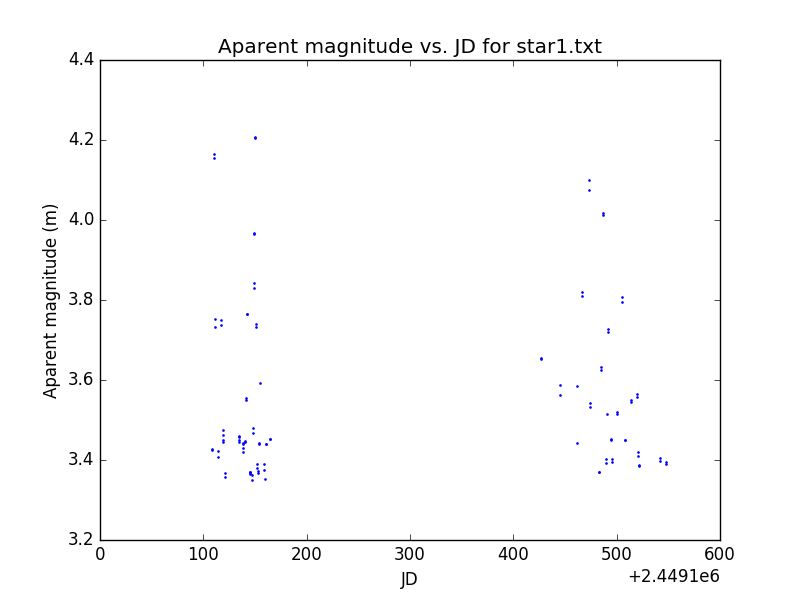
\includegraphics[scale=0.5]{star1txt_simple_plot.png}
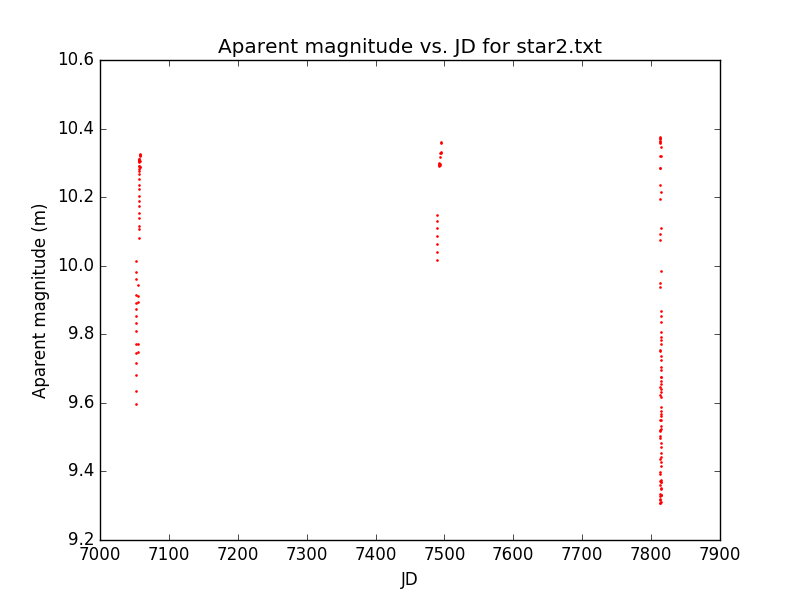
\includegraphics[scale=0.5]{star2txt_simple_plot.png}
\caption{This plots illustrate magnitude ($m_V$) vs. time $(JD)$ for the named files. \textit{Top}: Plot for \texttt{star1.txt}. \textit{Bottom}: Plot for \texttt{star2.txt}.} 
\label{fig:F1}
% SOURCE: /home/patricio/ast/esp01/code/lib/python/xkcd/paperwritting.py
\end{figure}


\item Phases have been computed using \href{https://www.univie.ac.at/tops/Period04/}{\texttt{Period04}} and its Fourier series method. Based on examples showed in class, I only decided to use 6 digits of the Phase. 

Results given by \texttt{Period04} are listed in Table \ref{table:period04calc}.

Figures 6 and 7: peroid and fit calculated by \texttt{Period04} for \texttt{star1.txt} (20 bins)  \& period and fit calculated by \texttt{Period04} for \texttt{star2.txt} (50 bins); respectively.    

\begin{figure}[tb]
\centering
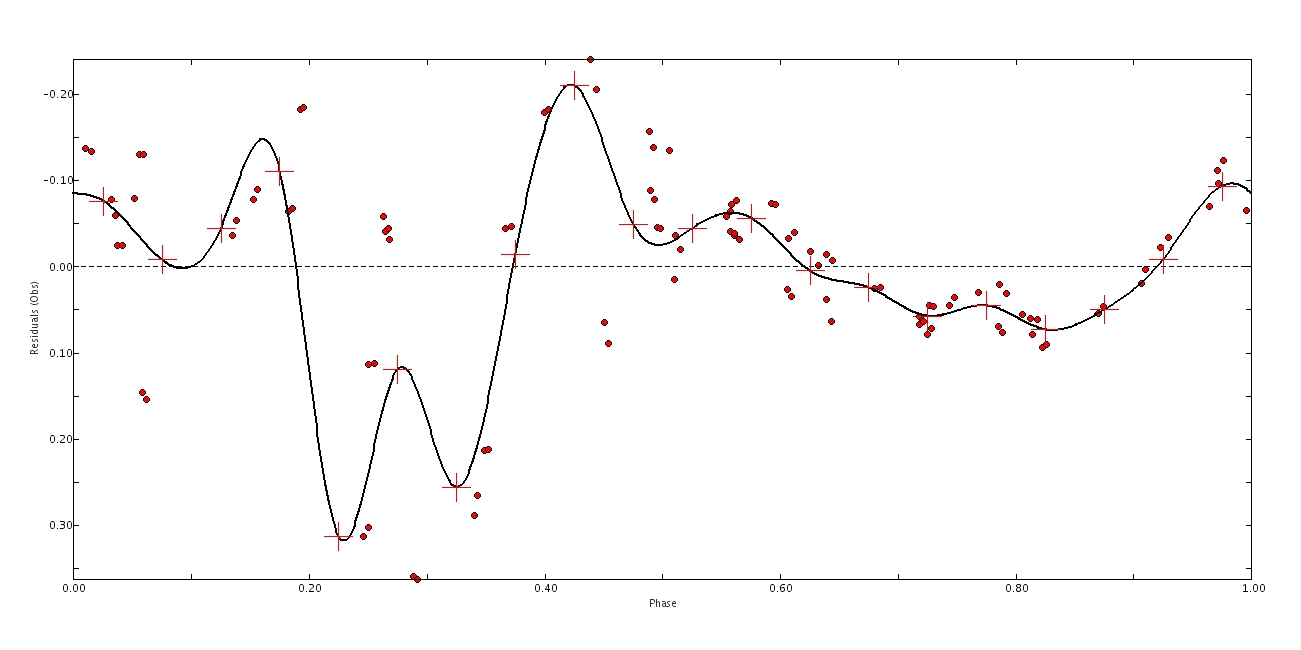
\includegraphics[width=\linewidth, clip]{star1txt_20bins.jpg}
\caption{Peroid and fit calculated by \texttt{Period04} for \texttt{star1.txt} with 20 bins thorugh Fourier series. Note that Y-axis has ``Residuals'' instead of apparent mags. $(m_V)$.}
\label{fig:F1}
% SOURCE: /home/patricio/ast/esp01/code/lib/python/xkcd/paperwritting.py
\end{figure}

\begin{figure}[tb]
\centering
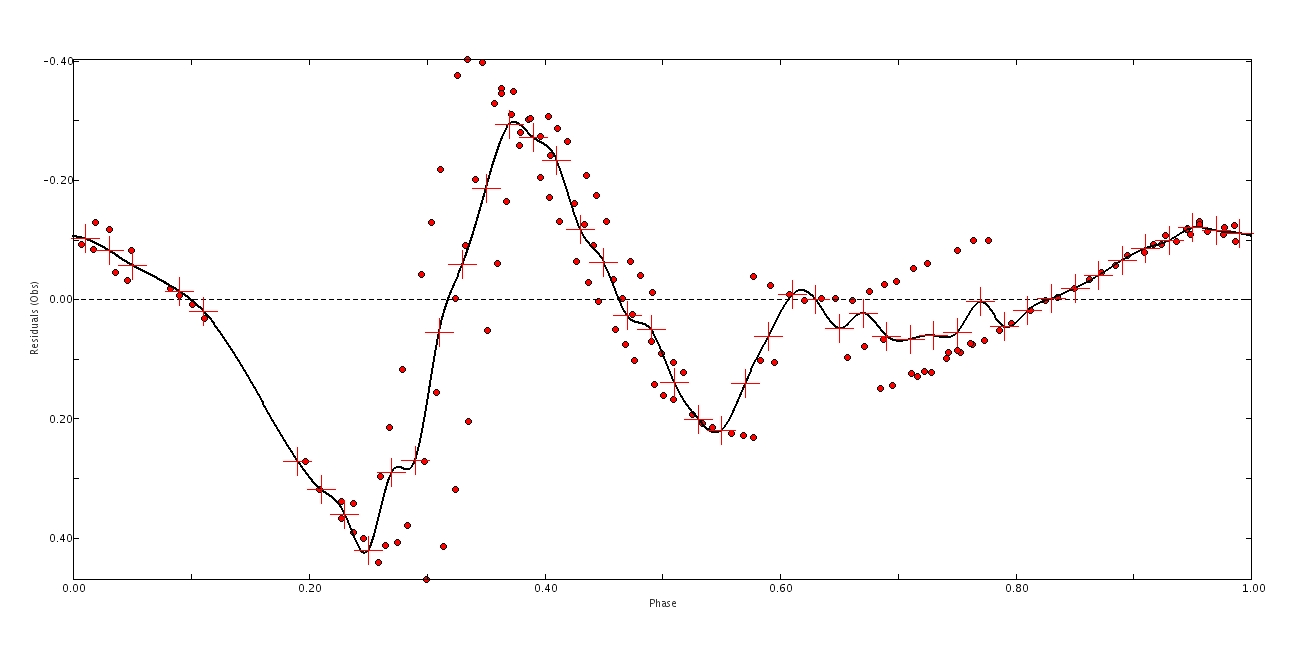
\includegraphics[width=\linewidth, clip]{star2txt_50bins.jpg}
\caption{Peroid and fit calculated by \texttt{Period04} for \texttt{star2.txt} with 50 bins thorugh Fourier series.}
\label{fig:F1}
% SOURCE: /home/patricio/ast/esp01/code/lib/python/xkcd/paperwritting.py
\end{figure}

\begin{figure}[tb]
\centering
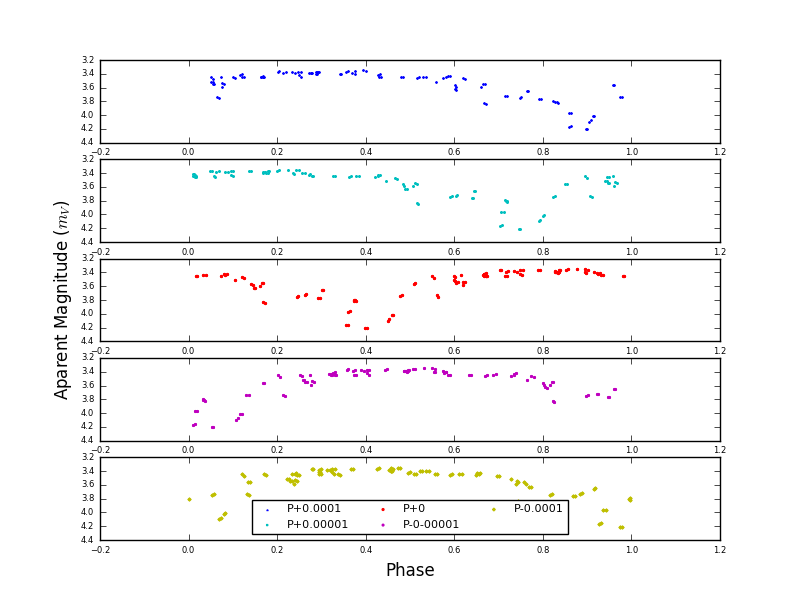
\includegraphics[scale=0.5]{star1txt_phase_quality.png}
\caption{Light curve for \texttt{star1.txt}. The main period here is $P_1 = 0.866062$. The number at the right of $+$ in plot legend says in how much I varied the period (in days).}
\label{fig:F1}
% SOURCE: /home/patricio/ast/esp01/code/lib/python/xkcd/paperwritting.py
\end{figure}

\begin{figure}[tb]
\centering
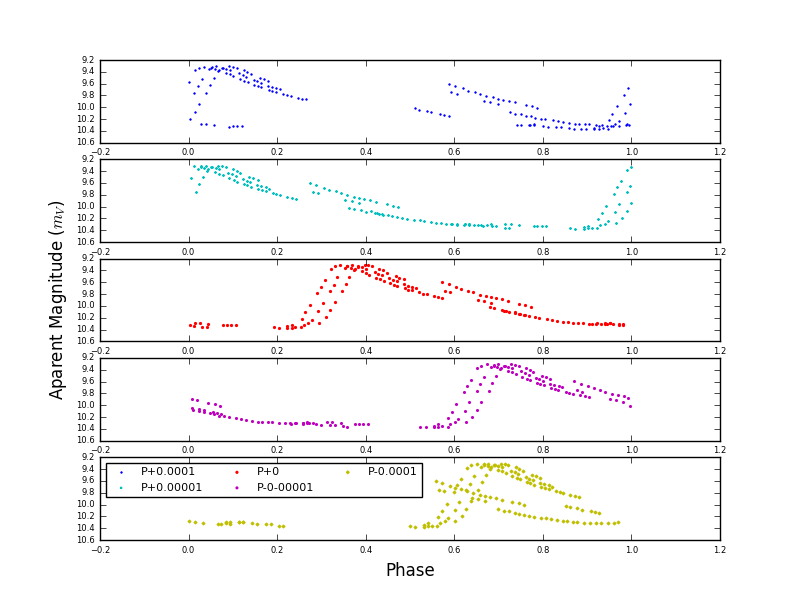
\includegraphics[scale=0.5]{star2txt_phase_quality.png}
\caption{Light curve for \texttt{star1.txt}. The main period here is $P_2 = 0.486062$. The number at the right of $+$ in plot legend says in how much I varied the period (in days).}
\label{fig:F1}
% SOURCE: /home/patricio/ast/esp01/code/lib/python/xkcd/paperwritting.py
\end{figure}

\item Here, as suggested in Homework instructions, I have changed a little the period and re-plotted apparent magnitude ($m_V$) vs. phase. I have changed the period found by \texttt{Period04} in $\pm 0.0001 (d)$ and $\pm 0.00001 (d)$, i.e., I changed the period in tiny amounts. This is plotted in Fig 8 and 9: apparent mag. ($V$) vs. phase for different periods for \texttt{star1.txt} \&  apparent mag. ($V$) vs. phase for different periods for \texttt{star2.txt}; respectively.

If the reader observe Figs. 8 and 9 it is really noticeable that with a little change in the period changes a lot the whole plot; somes becoming ``dubious''. This means that period found by \texttt{Period04} is quite good. The only problem I see is in Fig. 9. Here  I see that a little change in the period (let's say that \texttt{star2.txt} original period is $P_2$ in days), specifically when $P = (P_2 + 0.00001) d$ is basically the same light curve but the ``bump'' in the magnitude is simply displaced through x-axis. Remember that periods for \texttt{star1.txt} ($P_1$) and \texttt{star2.txt} ($P_2$) are in Table \ref{table:period04calc}.



\item Here, I'm trying to classify stars variability type knowing that their period is acceptable. For this classification I'm highly based in plots of different variable stars shown in classes and, also, looking for a pattern in the light curves. The star from \texttt{star1.txt} (hereafter, S1) doesn't have like a constant ``amplitude'' if we mentally fit a sine curve on it. The same applies to star from \texttt{star2.txt} (hereafter, S2). However, S1 light surve seems to have a ``wave'' pattern on it, i.e., I can see some cycles on it (this might be a lineal combination of sines and cosines). On the other hand, S2 light curve only has a ``bump'' on it's brightness (suddenly, apparent magnitude decreases; which means it is apparently brighter) and then its magnitude increases; also, and I don't see a clear pattern on it.

\begin{figure}[tb]
\centering
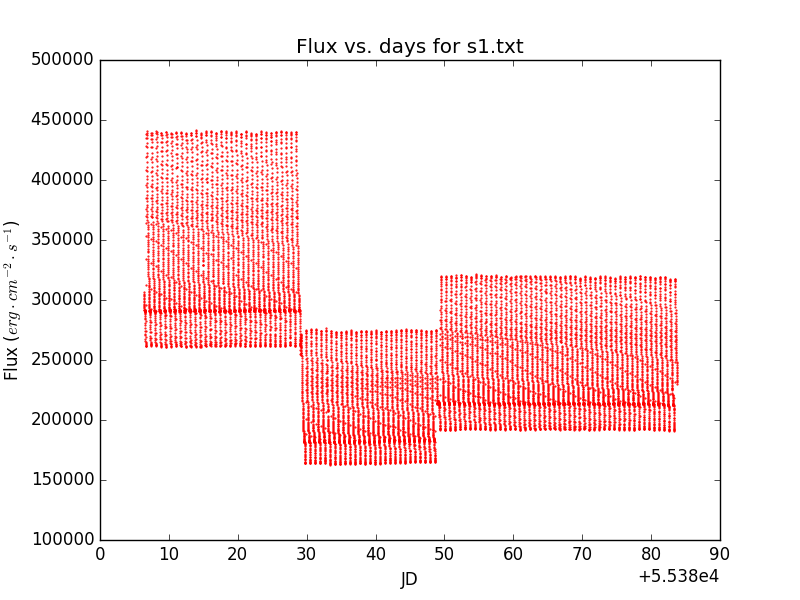
\includegraphics[scale=0.5]{s1txt_simple_plot.png}
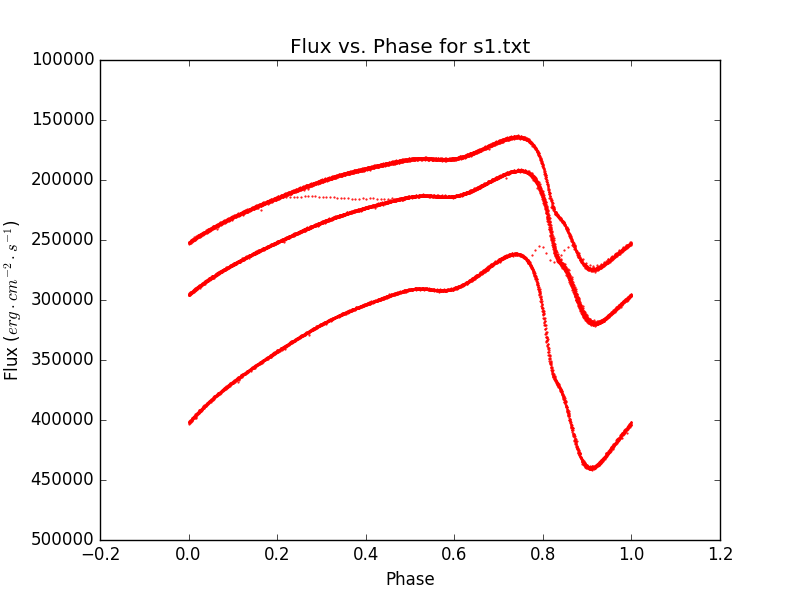
\includegraphics[scale=0.5]{s1txt_phase_plot.png}
\caption{\textit{Top}: Flux vs. time plot for IS1 file. \textit{Bottom}: Light curve for IS1 file. This figure shows that, for this period ($P =0.723708 d$) something that seems like 3 different stars, which is weird.}
\label{fig:F1}
% SOURCE: /home/patricio/ast/esp01/code/lib/python/xkcd/paperwritting.py
\end{figure}


Based on this is that I think the first star, S1, is an \emph{eclipsing binary variable}. Mainly because it shows a pattern of its changing magnitude. Of course, this is not a perfect sine or cosine function (if we fit an imaginary fit), but, as said, it has a clear pattern. I decided to discard a pulsating or rotating star because its changes in brightness is not so constant in amplitude. This could be because the object orbiting between the star and our vision range is not perfectly aligned with us.

The second star I think is clearly an \emph{eruptive variable}. As said, suddenly this star increases its brightness. This could be because of violent events occurring in this star. I discarded that this could be a cataclysmic variable because its brightness doesn't increases excessively. But, of course, this last reason isn't enough. S2 file gives apparent magnitude and if the object is too far it might be a cataclysmic.

\begin{figure}[tb]
\centering
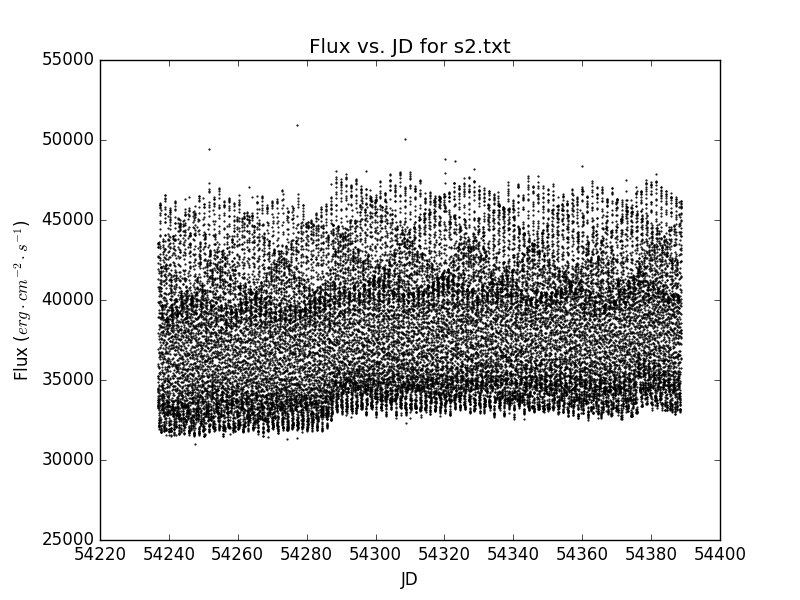
\includegraphics[scale=0.5]{s2txt_simple_plot.png}
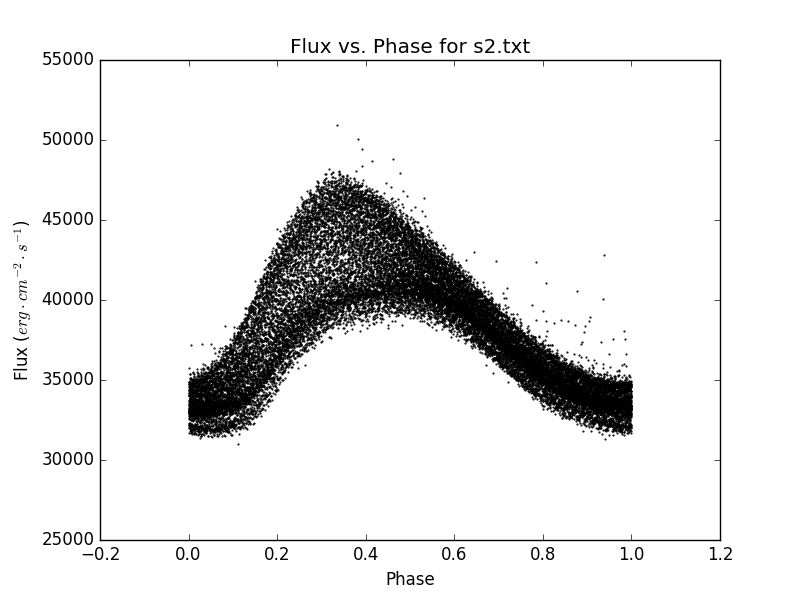
\includegraphics[scale=0.5]{s2txt_phase_plot.png}
\caption{\textit{Top}: Flux vs. time plot for IS1 file. \textit{Bottom}: Light curve for IS1 file. This figure shows that, for this period ($P =0.363625 d$). This could be a multiperiodic star because, if we pay attention, its waveform is very thick. }
\label{fig:F1}
% SOURCE: /home/patricio/ast/esp01/code/lib/python/xkcd/paperwritting.py
\end{figure}

\end{enumerate}
\section{Fourth Problem: Multiperiodic stars}

From \href{http://idoc-corot.ias.u-psud.fr/}{IAS CoRoT Public Archive} I download data for two stars, hereafter called IS1 (for the first star, with ID 0105173544) and IS2 (for the second star, with ID 0101368812). The difference between these stars and stars in the third problem lies in the stars of this problem are space-base observed. While S1 and S2 are ground-based observed.

\begin{enumerate} [a)]
\item The results for IS1 is plotted and illustrated in Fig. 10. I decided to calculate Fourier for the period using ``Residual Adjusted'' option in \texttt{Period04}. I did this because, when I computed Fourier using ``Original Data'' option the period computed was terrible. But when I computed it using the option indicated above a more acceptable period was found. However, the plot shown in Fig. 10 (bottom) is strange since it has 3 sequences. The period found for IS1 was $P_{IS1} = 0.723708 d$. The other candidate for the period was $\tilde{P_{IS1}} = 96.750655 d$.


\item IS2 plots are in Fig. 11. Is this a multiperiodic star? I think yes, it is. Why? Clearly we can see in Fig. 13 a great period, with its peak at phase $\varphi \sim 0.33  $. But, also, this great ``wave'' form is very thick. So thick that it could mean that it thickness is caused by very little ``wave forms'' or variability/pulsations (I also go deeper about this in the next subitem).

\item Figure 12 is divided into two subfigures, but both are the same: the Power Spectrum of IS2. Top image shows the whole Power Spectrum while the bottom image shows the ``peaks'' found by \texttt{Period04} Fourier method. So, prewhitening is basically delete the greater peak (Fig. 12 at the bottom) and recalculate it's period with the smaller ``peaks''. But, unfortunately, I didn't find how to do this in \texttt{Period04} (even searching in \texttt{Period 04 Manual Tutorial} about prewhitining it doesn't say exactly how to do it). My apologies if I could not do it. But I tried using \texttt{Period04} and \texttt{IRAF PDM} and I didn't find how to do it in both. However, I want to emphasize that Fig. 12 shows that we have clearly more than one ``peak'' and that means that IS2 has more than one period; therefore it is a multiperiodic variable star.

As suggested and showed by \href{https://www.aanda.org/articles/aa/pdf/2009/05/aa11441-08.pdf}{Olech \& Moskalik (2008)} prewhitening is vital to find periods with lower amplitud that are opaqued by the ``main'' amplitude. That's how, for example, in an iterative method of prewhitening they find 6 double mode RR Lyrae pulsators; 2 of them being classified as a new member of double mode RR Lyrae pulsators. 

\begin{figure}[tb]
\centering
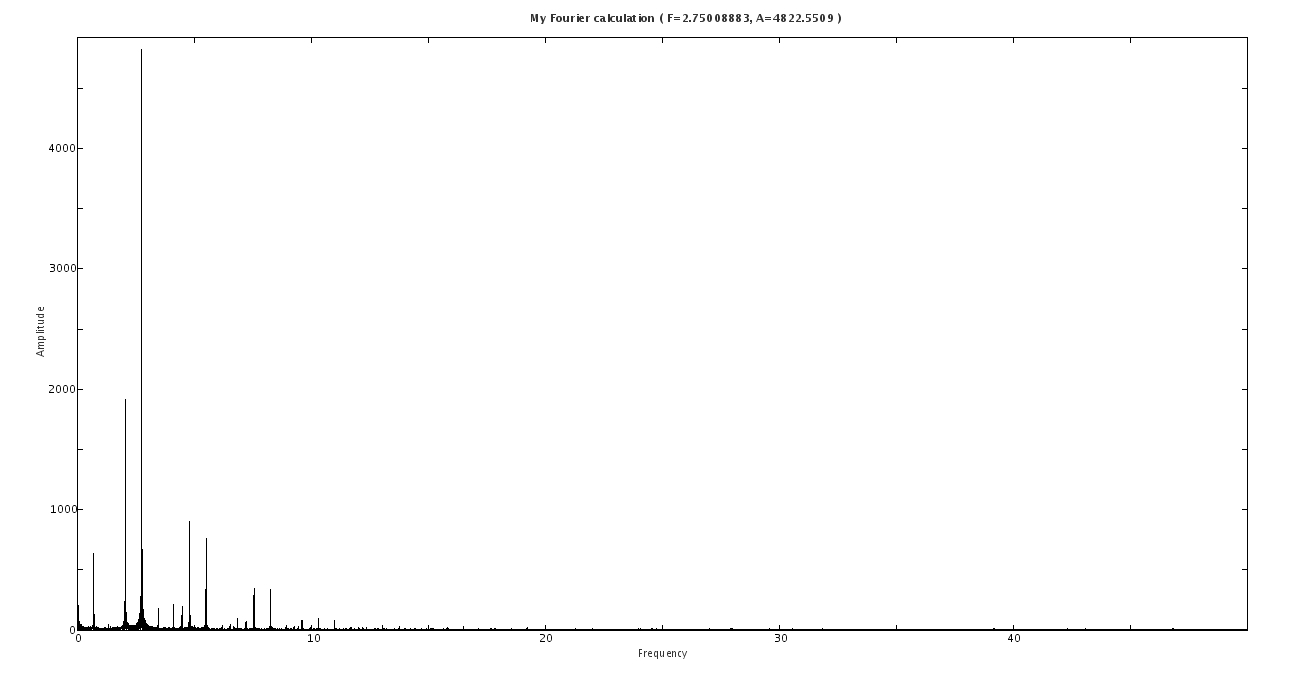
\includegraphics[scale=0.2]{Power_Spectrum_s2_0.jpg}
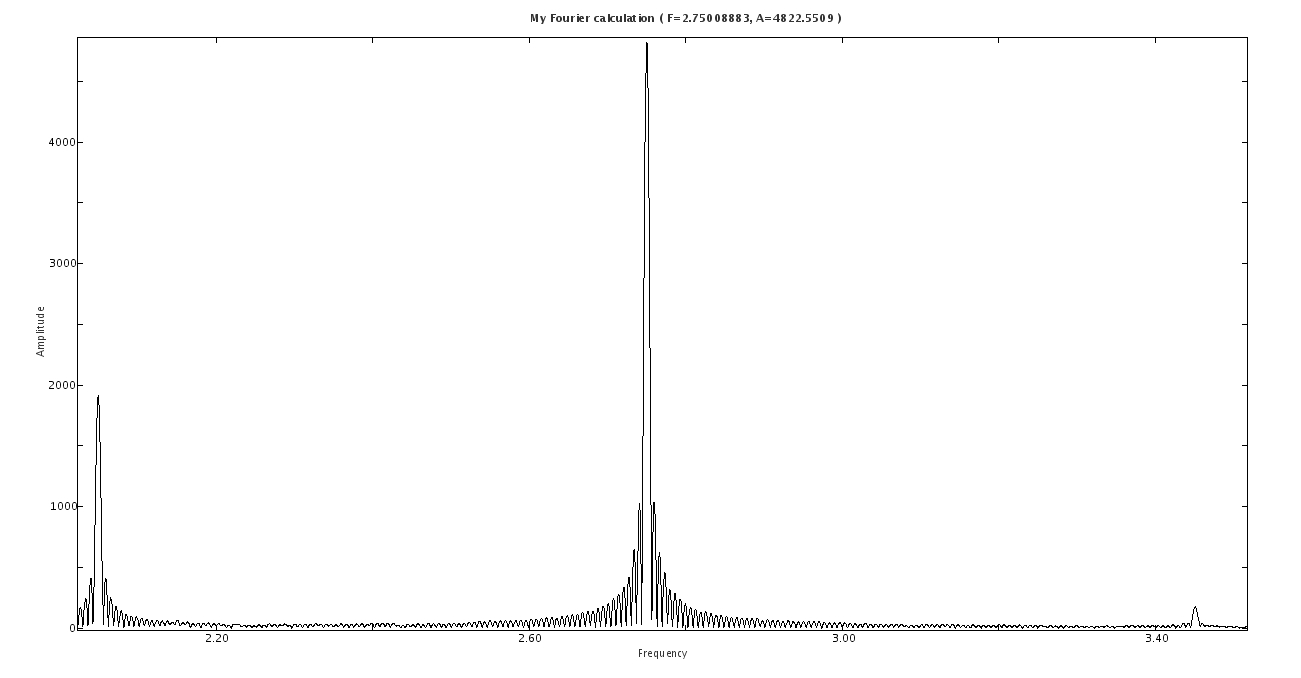
\includegraphics[scale=0.2]{Power_Spectrum_s2.jpg}
\caption{\textit{Top}: Power Spectrum for IS2.
\textit{Bottom}: Power Spectrum for IS2 zoomed in range of frequencies $\sim [2.0, 3.6]$. Both images were obtanied using \texttt{Period04}.}
\label{fig:F1}
% SOURCE: /home/patricio/ast/esp01/code/lib/python/xkcd/paperwritting.py
\end{figure}
\end{enumerate}

\end{document}
